% !TEX root = ../thesis.tex
%
\chapter{Wyniki}
\label{sec:wyniki_eksperymentow}

W niniejszym rozdziale przedstawiono wynik działania programu \texttt{mostitch} na trzech przykładowych zbiorach angiograficznych obrazów OCT dostarczonych w ramach projektu RIMO-BIOL (sekcja \ref{sec:wstep:rimo-biol}). Wynik działania programu na zbiorze to cztery mozaiki powzstałę za pomocą różnych kombinacji wartości parametrów (proces opisano w \ref{sec:proponowane_algorytmy:proces_decyzyjny}):

\begin{enumerate}
\item \textbf{Wersja 1} -- \texttt{simplerTransform = false}, \texttt{rigidTransform = true}, \texttt{usePaths = false}. 
\item \textbf{Wersja 2} -- \texttt{simplerTransform = true}, \texttt{rigidTransform = true}, \texttt{usePaths = true}.
\item \textbf{Wersja 3} -- \texttt{simplerTransform = true}, \texttt{rigidTransform = true}, \texttt{usePaths = false}.
\item \textbf{Wersja 4} -- \texttt{simplerTransform = true}, \texttt{rigidTransform = false}, \texttt{usePaths = false}.
\end{enumerate}

\section{Zbiór 1}
\label{sec:zbior_1}

Rysunek \ref{fig:wyniki_eksperymentow:zbior_1} przedstawia zbiór angiograficznych obrazów OCT, natomiast rysunek \ref{fig:wyniki_eksperymentow:wynik_zbior_1} przedstawia wynik działania programu \texttt{mostitch}.

\begin{figure}[H]
  \centering
  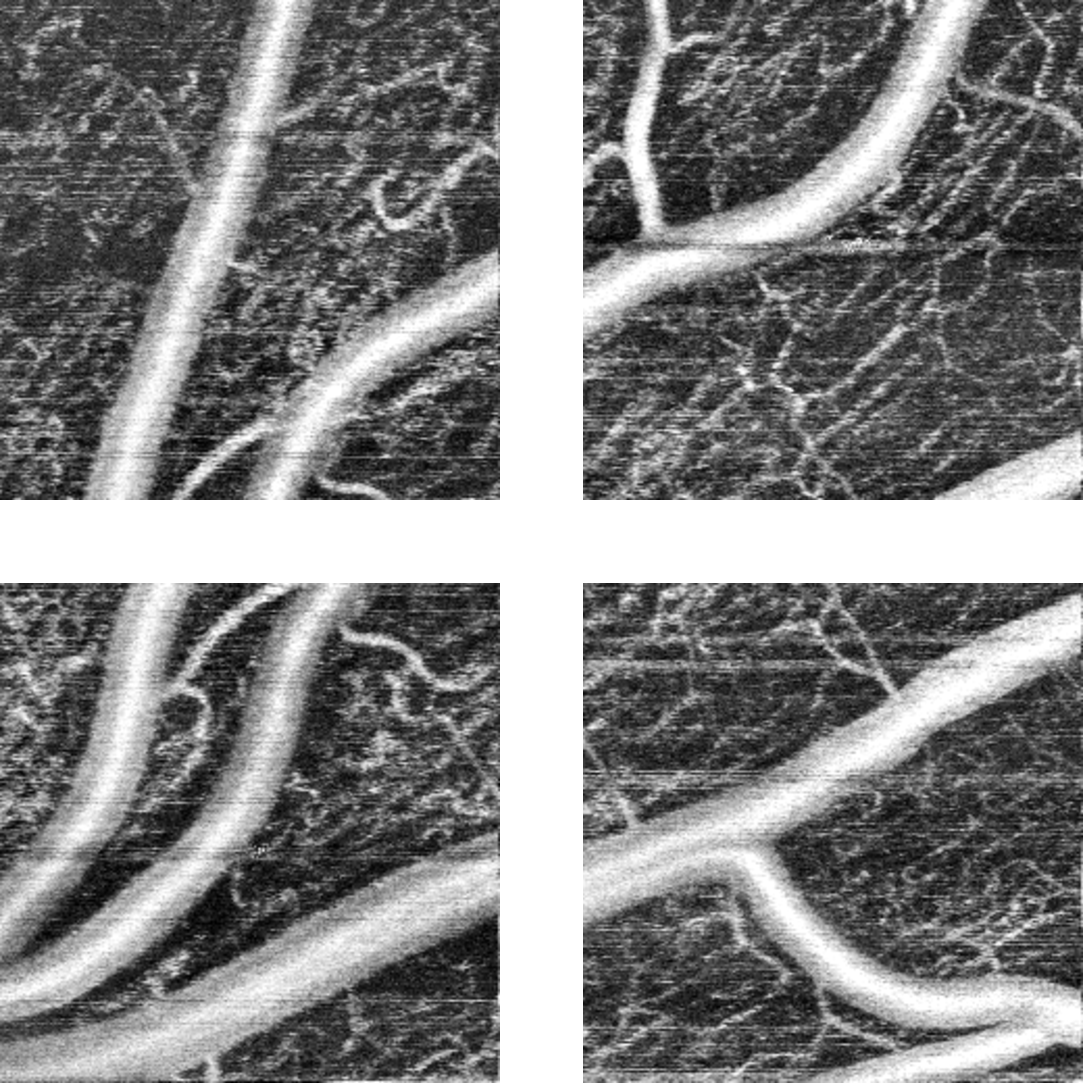
\includegraphics[width=5cm]{gfx/zbior_1}
  \caption{Przykładowy zbiór angiograficznych obrazów OCT umieszczonych zgodnie z ich współrzędnymi. Obraz referencyjny znajduje się w prawym górnym rogu.}
  \label{fig:wyniki_eksperymentow:zbior_1}
\end{figure}

\begin{figure}[htb]
  \centering
  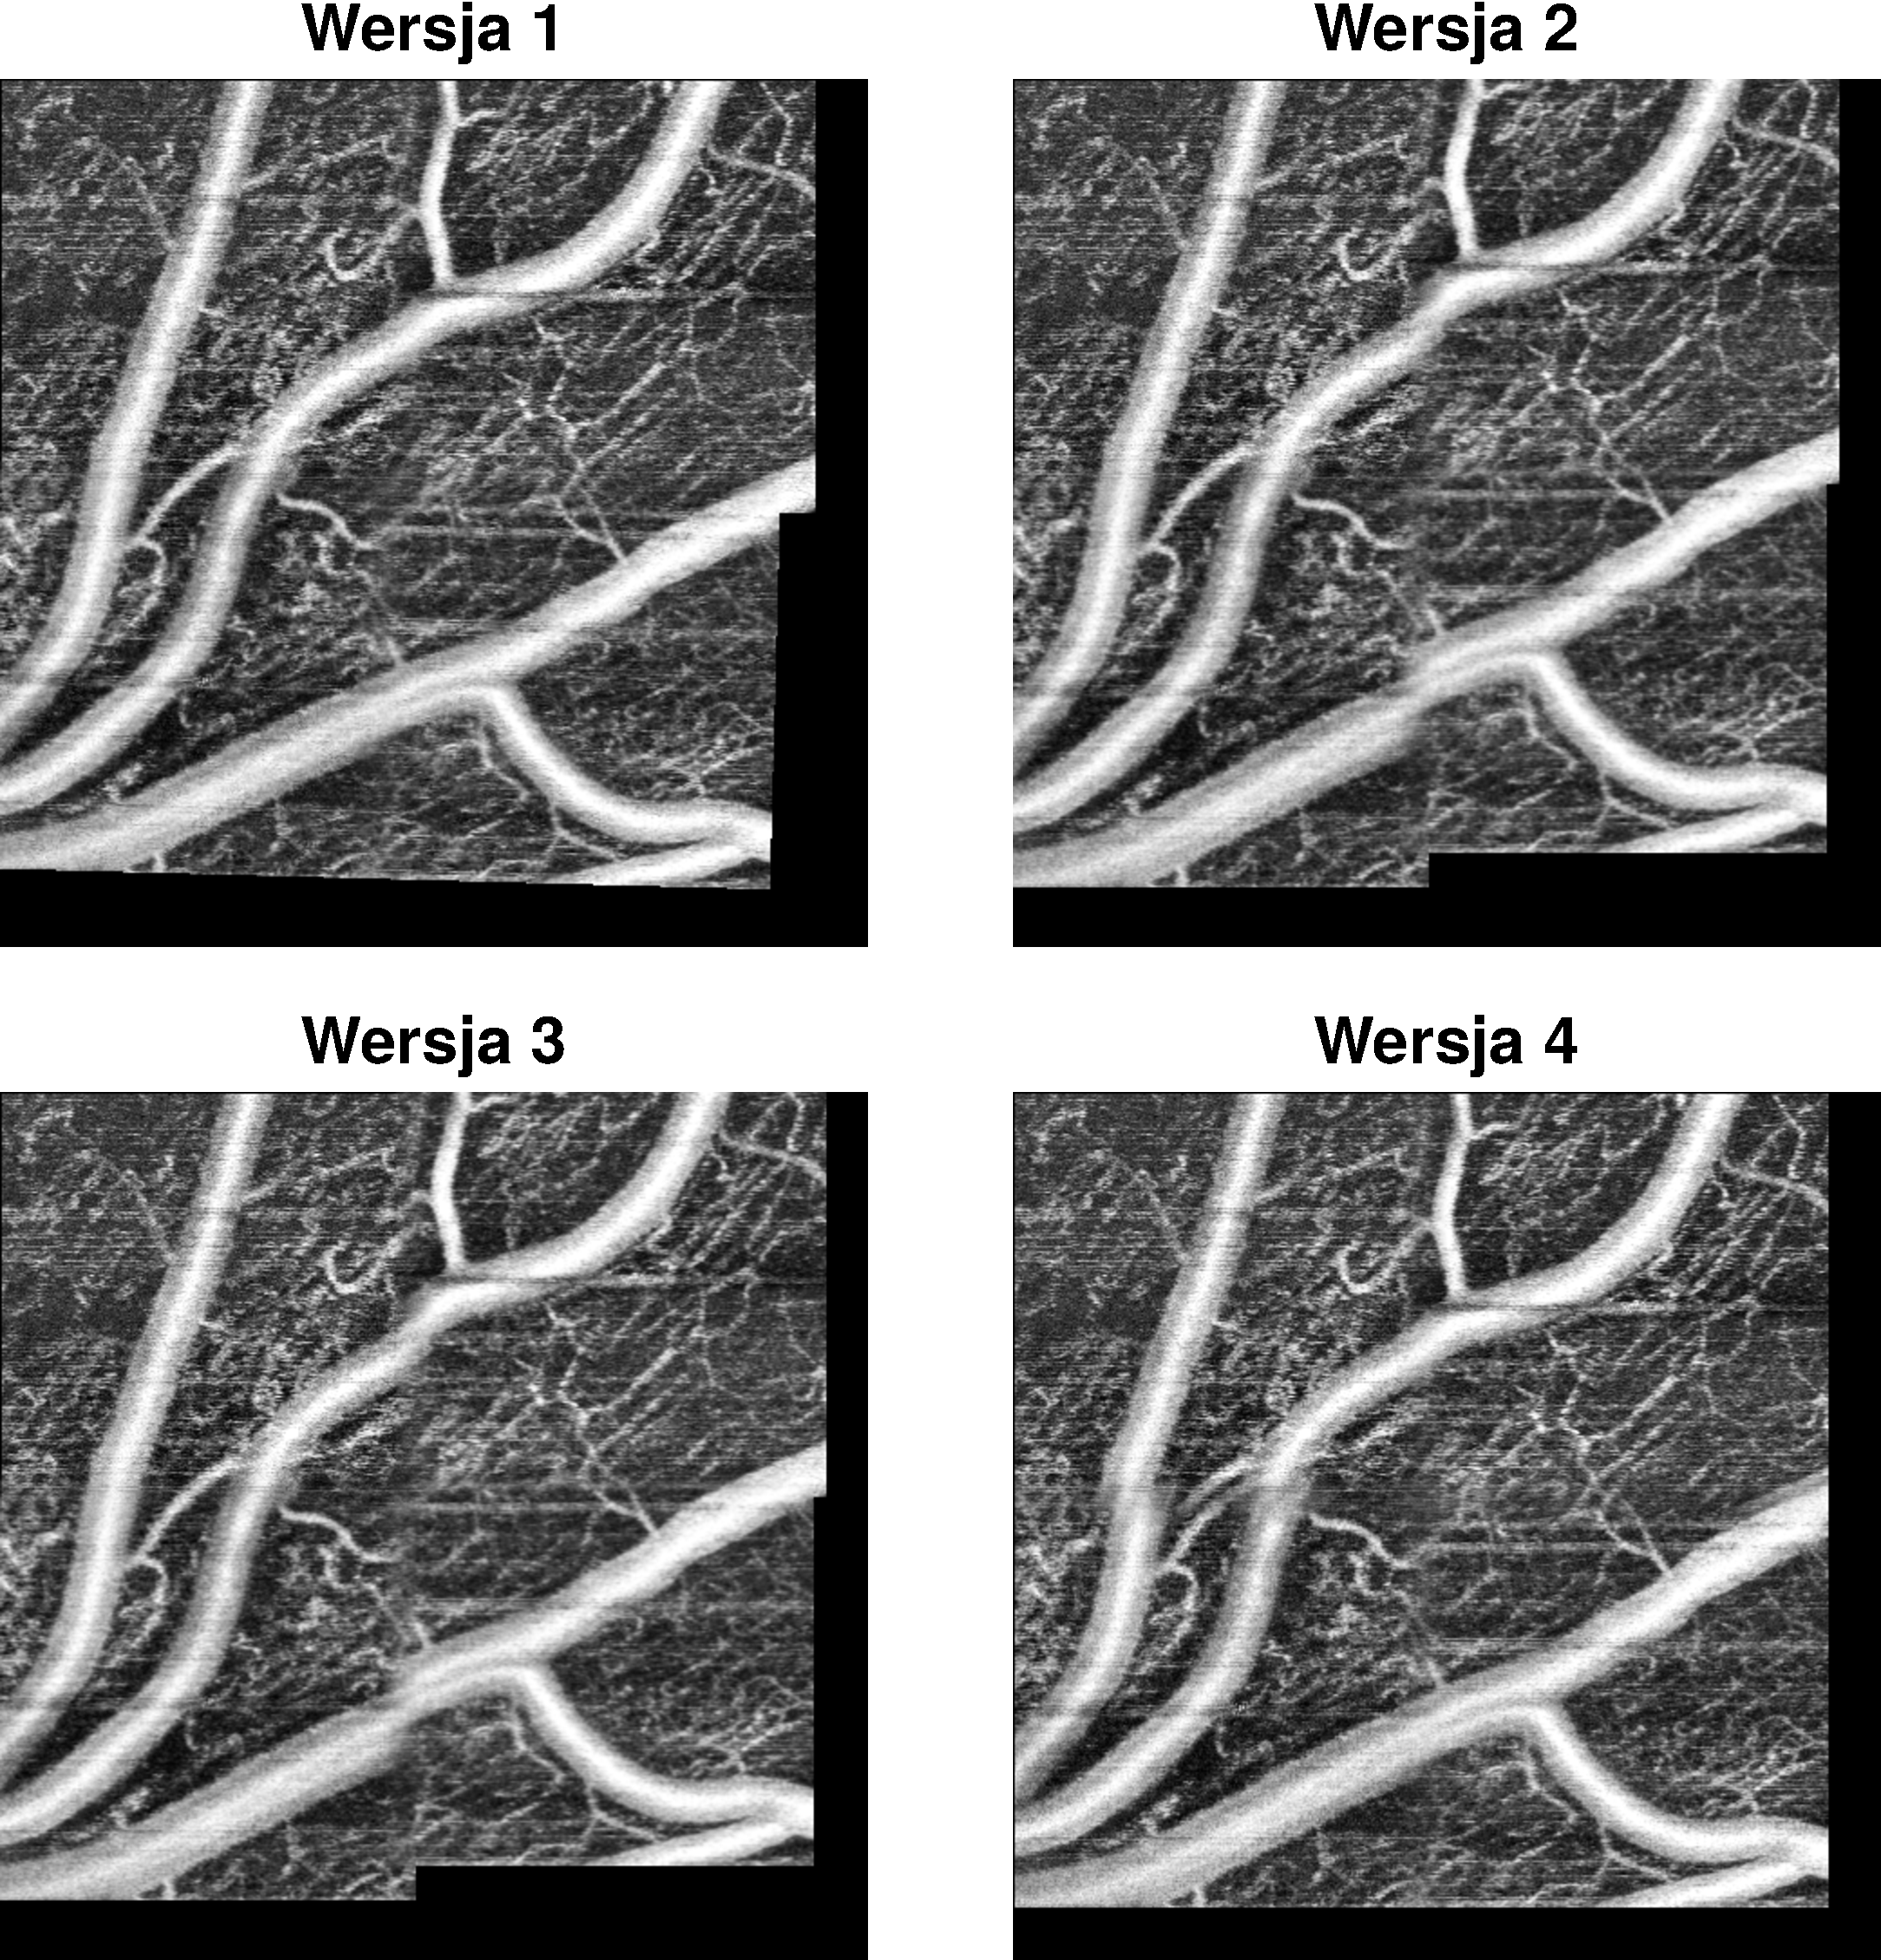
\includegraphics[width=10cm]{gfx/wynik_zbior_1}
  \caption{Cztery mozaiki będą wynikiem działania programu \texttt{mostitch} na zbiorze obrazów OCT z rysunku \ref{fig:wyniki_eksperymentow:zbior_1}.}
  \label{fig:wyniki_eksperymentow:wynik_zbior_1}
\end{figure}

\section{Zbiór 2}
\label{sec:zbior_2}

Rysunek \ref{fig:wyniki_eksperymentow:zbior_2} przedstawia zbiór angiograficznych obrazów OCT, natomiast rysunek \ref{fig:wyniki_eksperymentow:wynik_zbior_2} przedstawia wynik działania programu \texttt{mostitch}.

\begin{figure}[H]
  \centering
  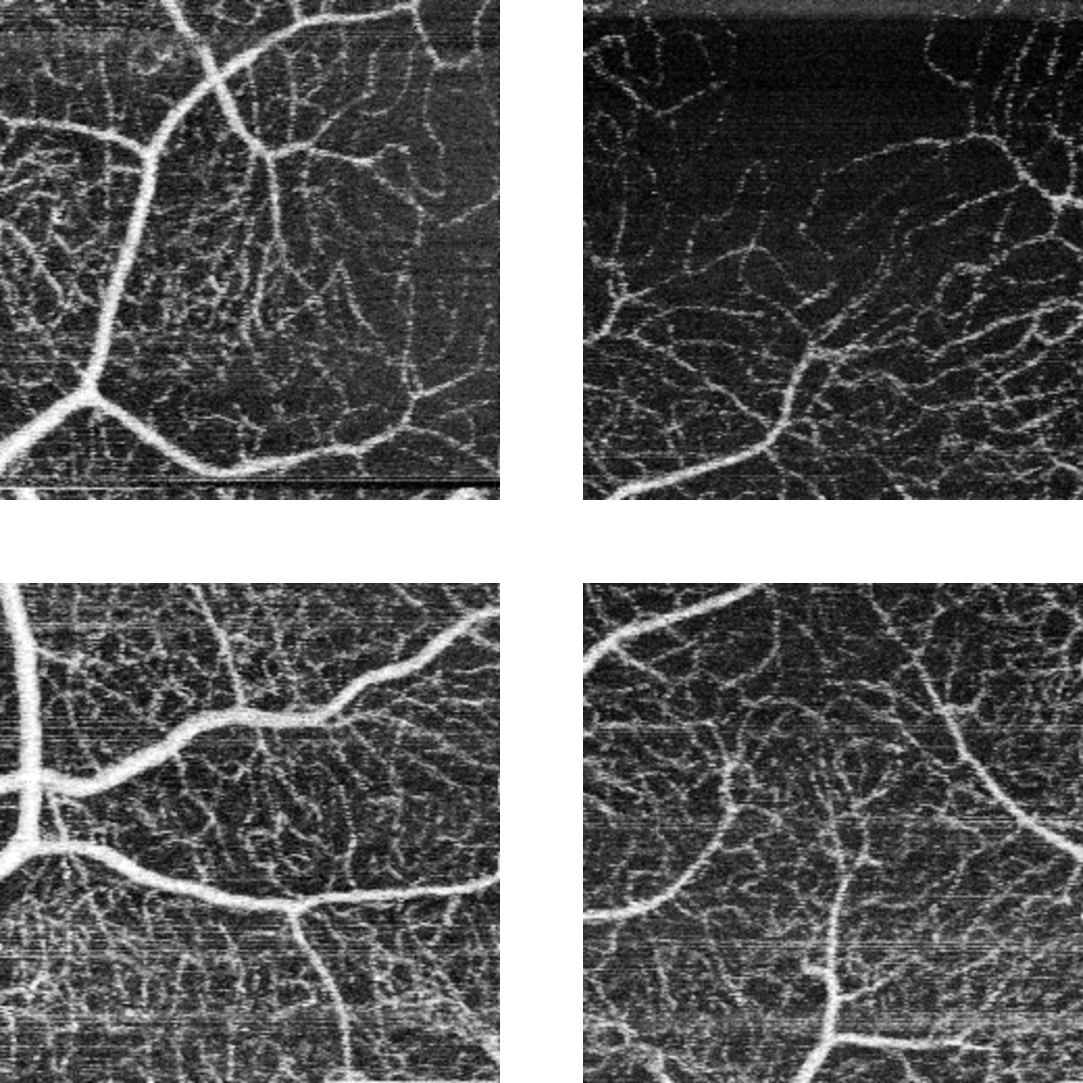
\includegraphics[width=5cm]{gfx/zbior_2}
  \caption{Przykładowy zbiór angiograficznych obrazów OCT umieszczonych zgodnie z ich współrzędnymi. Obraz referencyjny znajduje się w prawym górnym rogu.}
  \label{fig:wyniki_eksperymentow:zbior_2}
\end{figure}

\begin{figure}[htb]
  \centering
  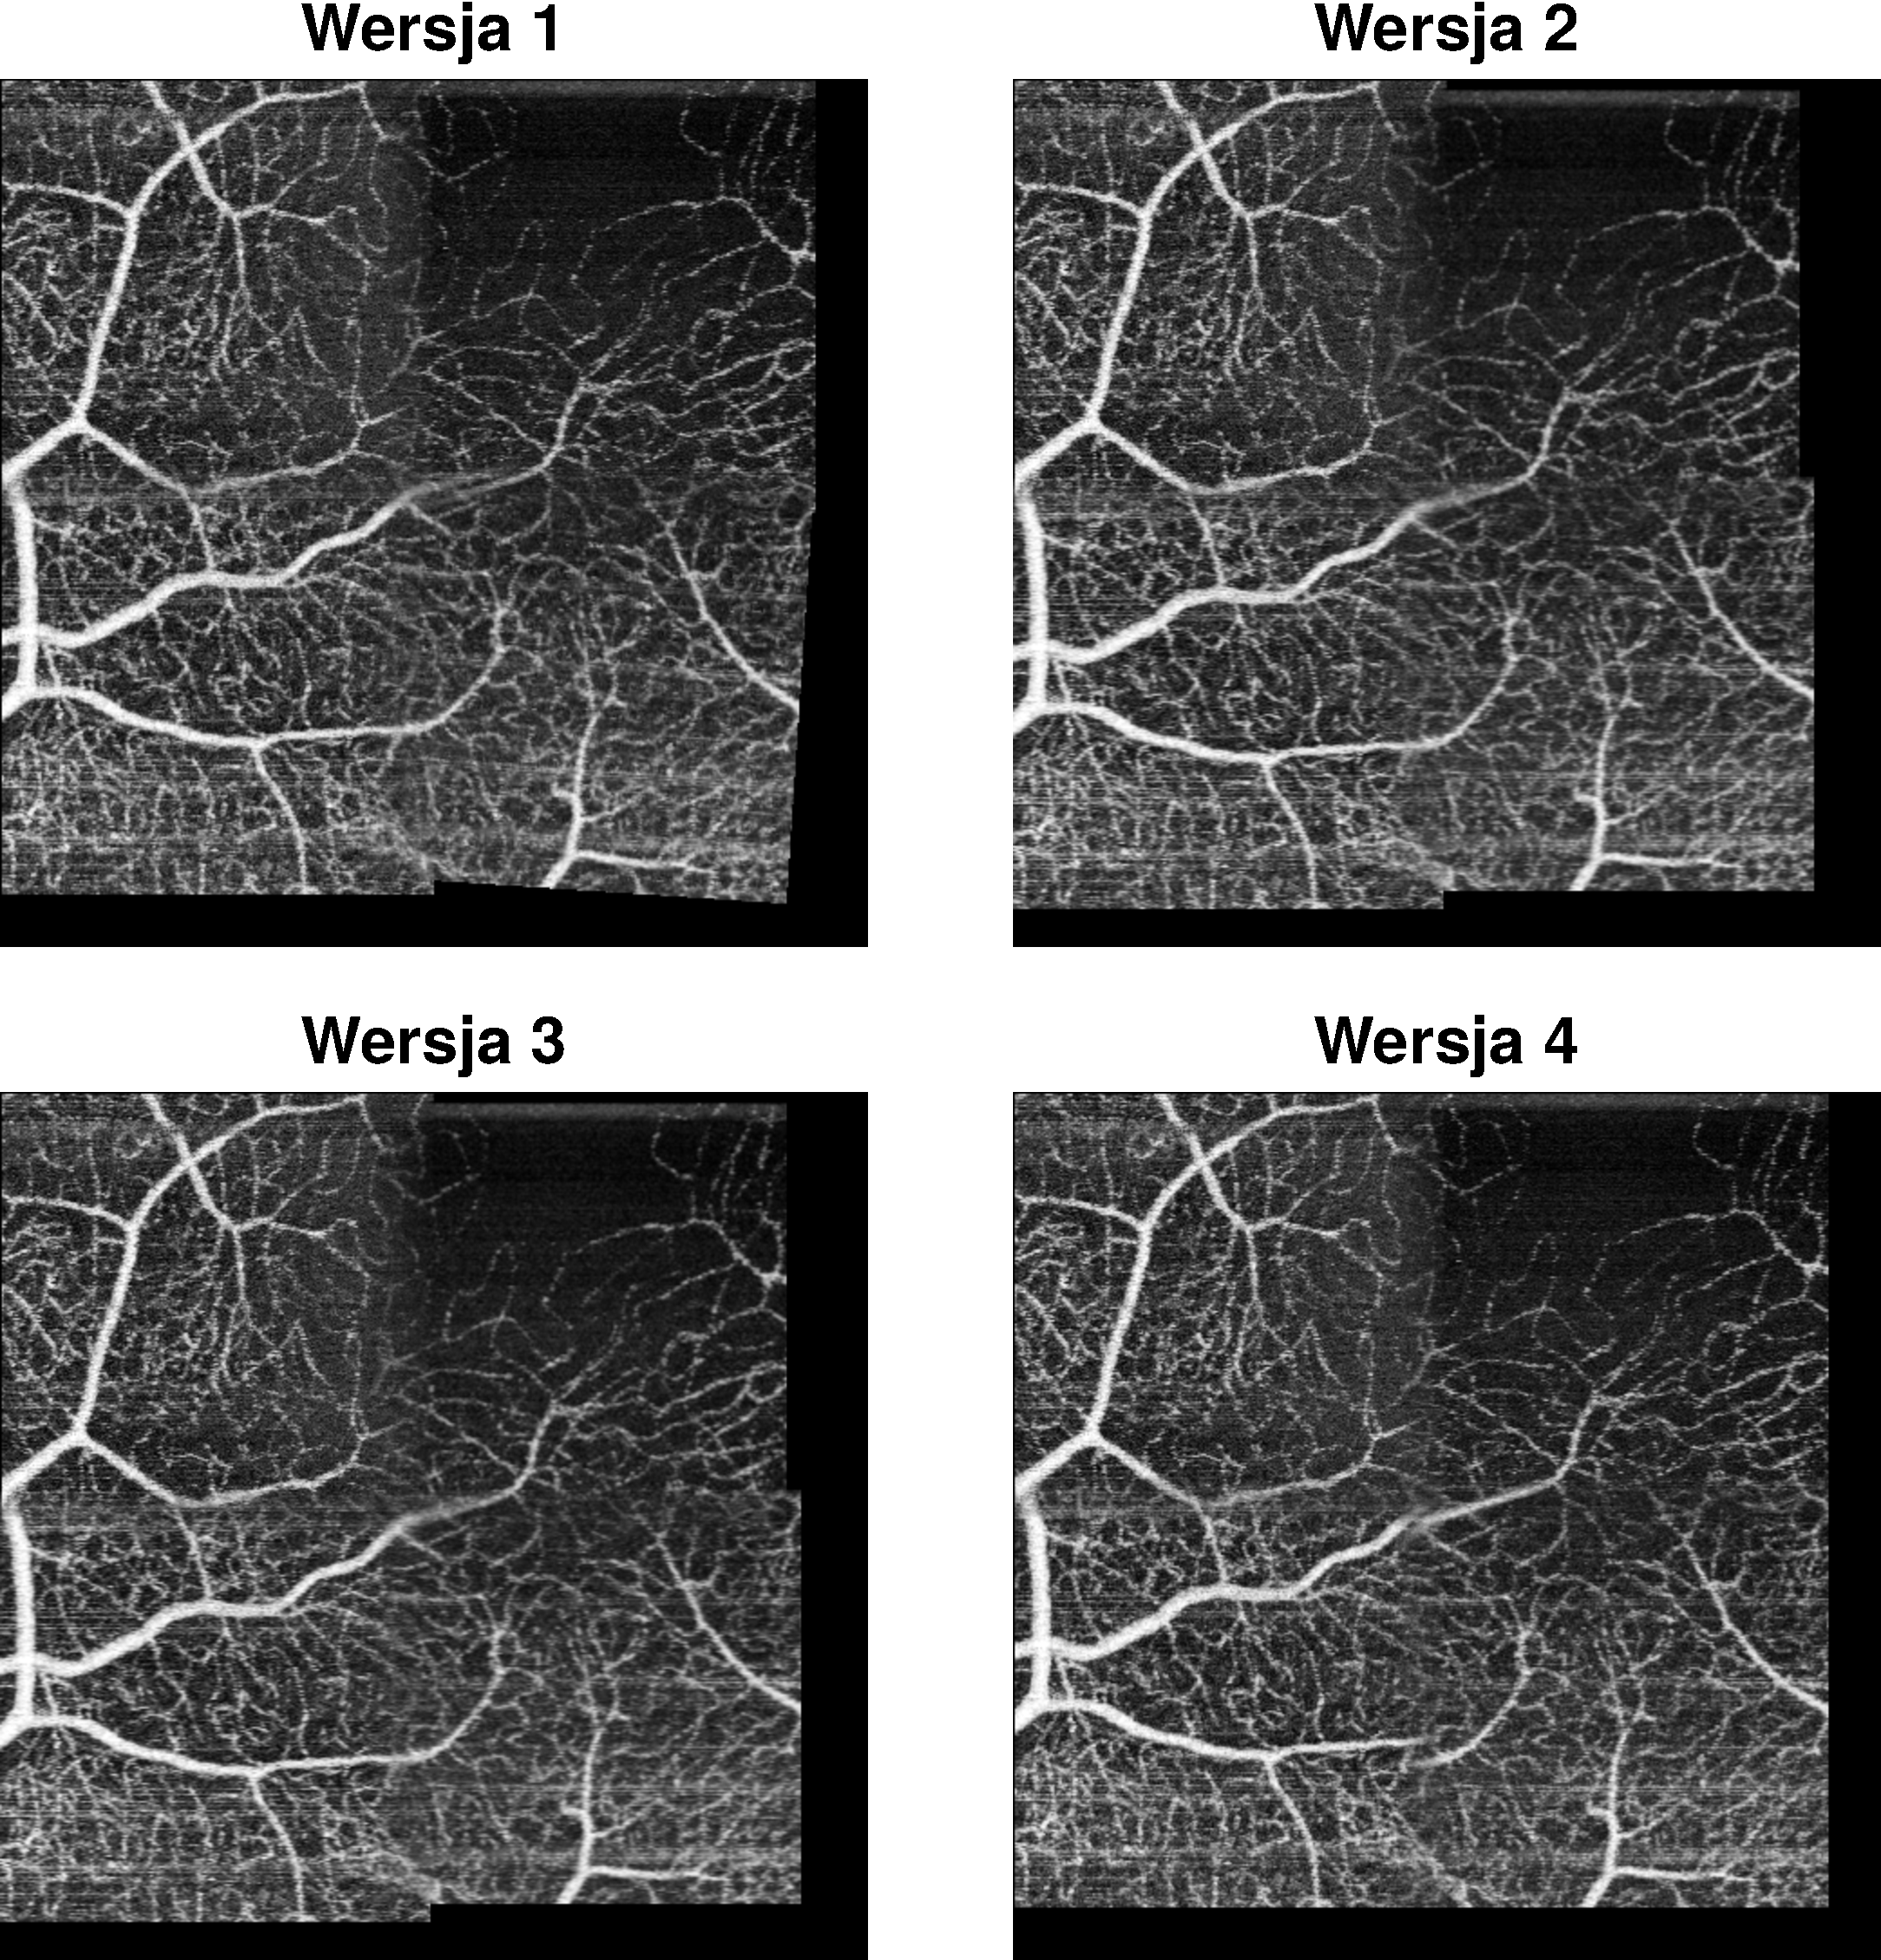
\includegraphics[width=10cm]{gfx/wynik_zbior_2}
  \caption{Cztery mozaiki będą wynikiem działania programu \texttt{mostitch} na zbiorze obrazów OCT z rysunku \ref{fig:wyniki_eksperymentow:zbior_2}.}
  \label{fig:wyniki_eksperymentow:wynik_zbior_2}
\end{figure}

\section{Zbiór 3}
\label{sec:zbior_3}

Rysunek \ref{fig:wyniki_eksperymentow:zbior_3} przedstawia zbiór angiograficznych obrazów OCT, natomiast rysunek \ref{fig:wyniki_eksperymentow:wynik_zbior_3} przedstawia wynik działania programu \texttt{mostitch}.

\begin{figure}[H]
  \centering
  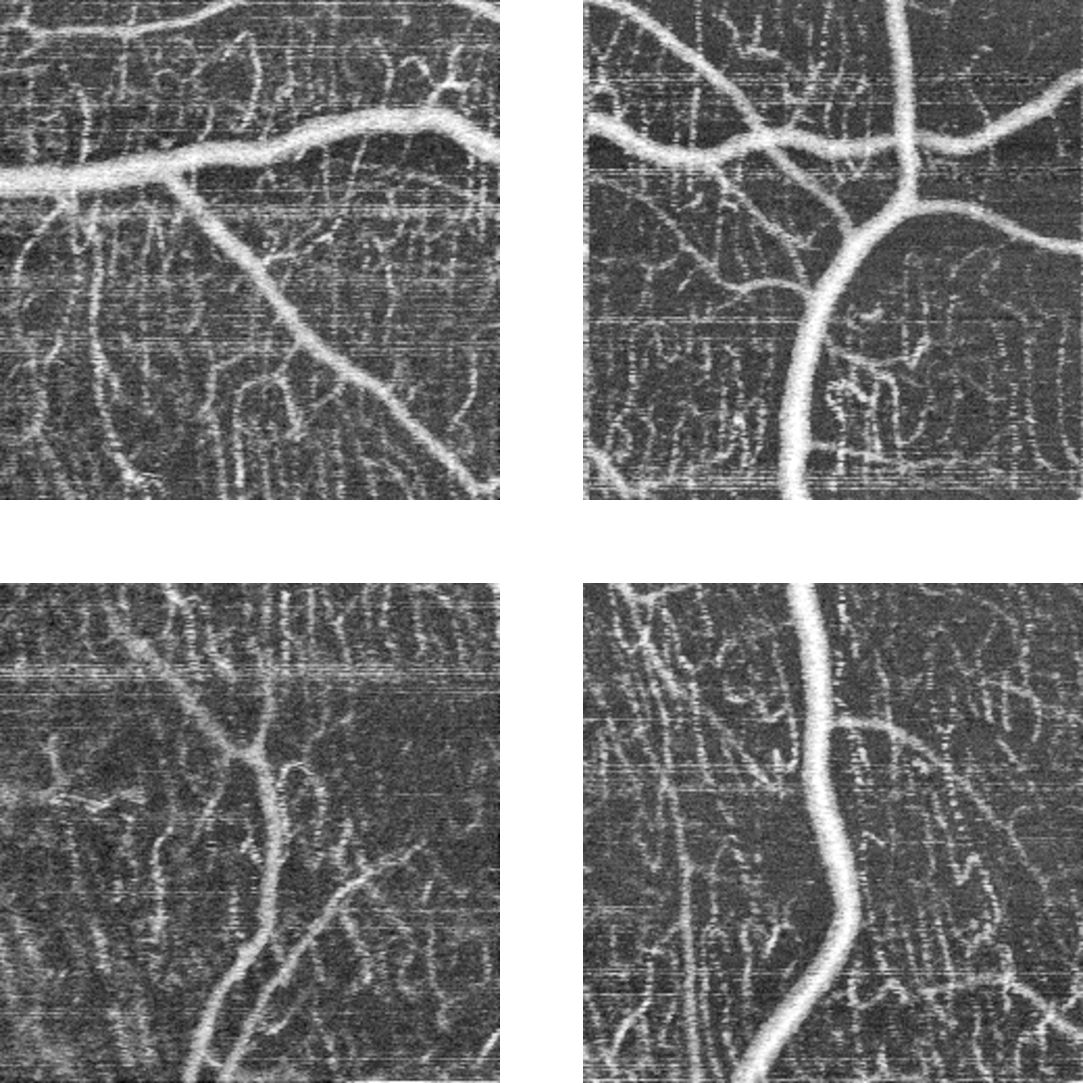
\includegraphics[width=5cm]{gfx/zbior_3}
  \caption{Przykładowy zbiór angiograficznych obrazów OCT umieszczonych zgodnie z ich współrzędnymi. Obraz referencyjny znajduje się w prawym górnym rogu.}
  \label{fig:wyniki_eksperymentow:zbior_3}
\end{figure}

\begin{figure}[htb]
  \centering
  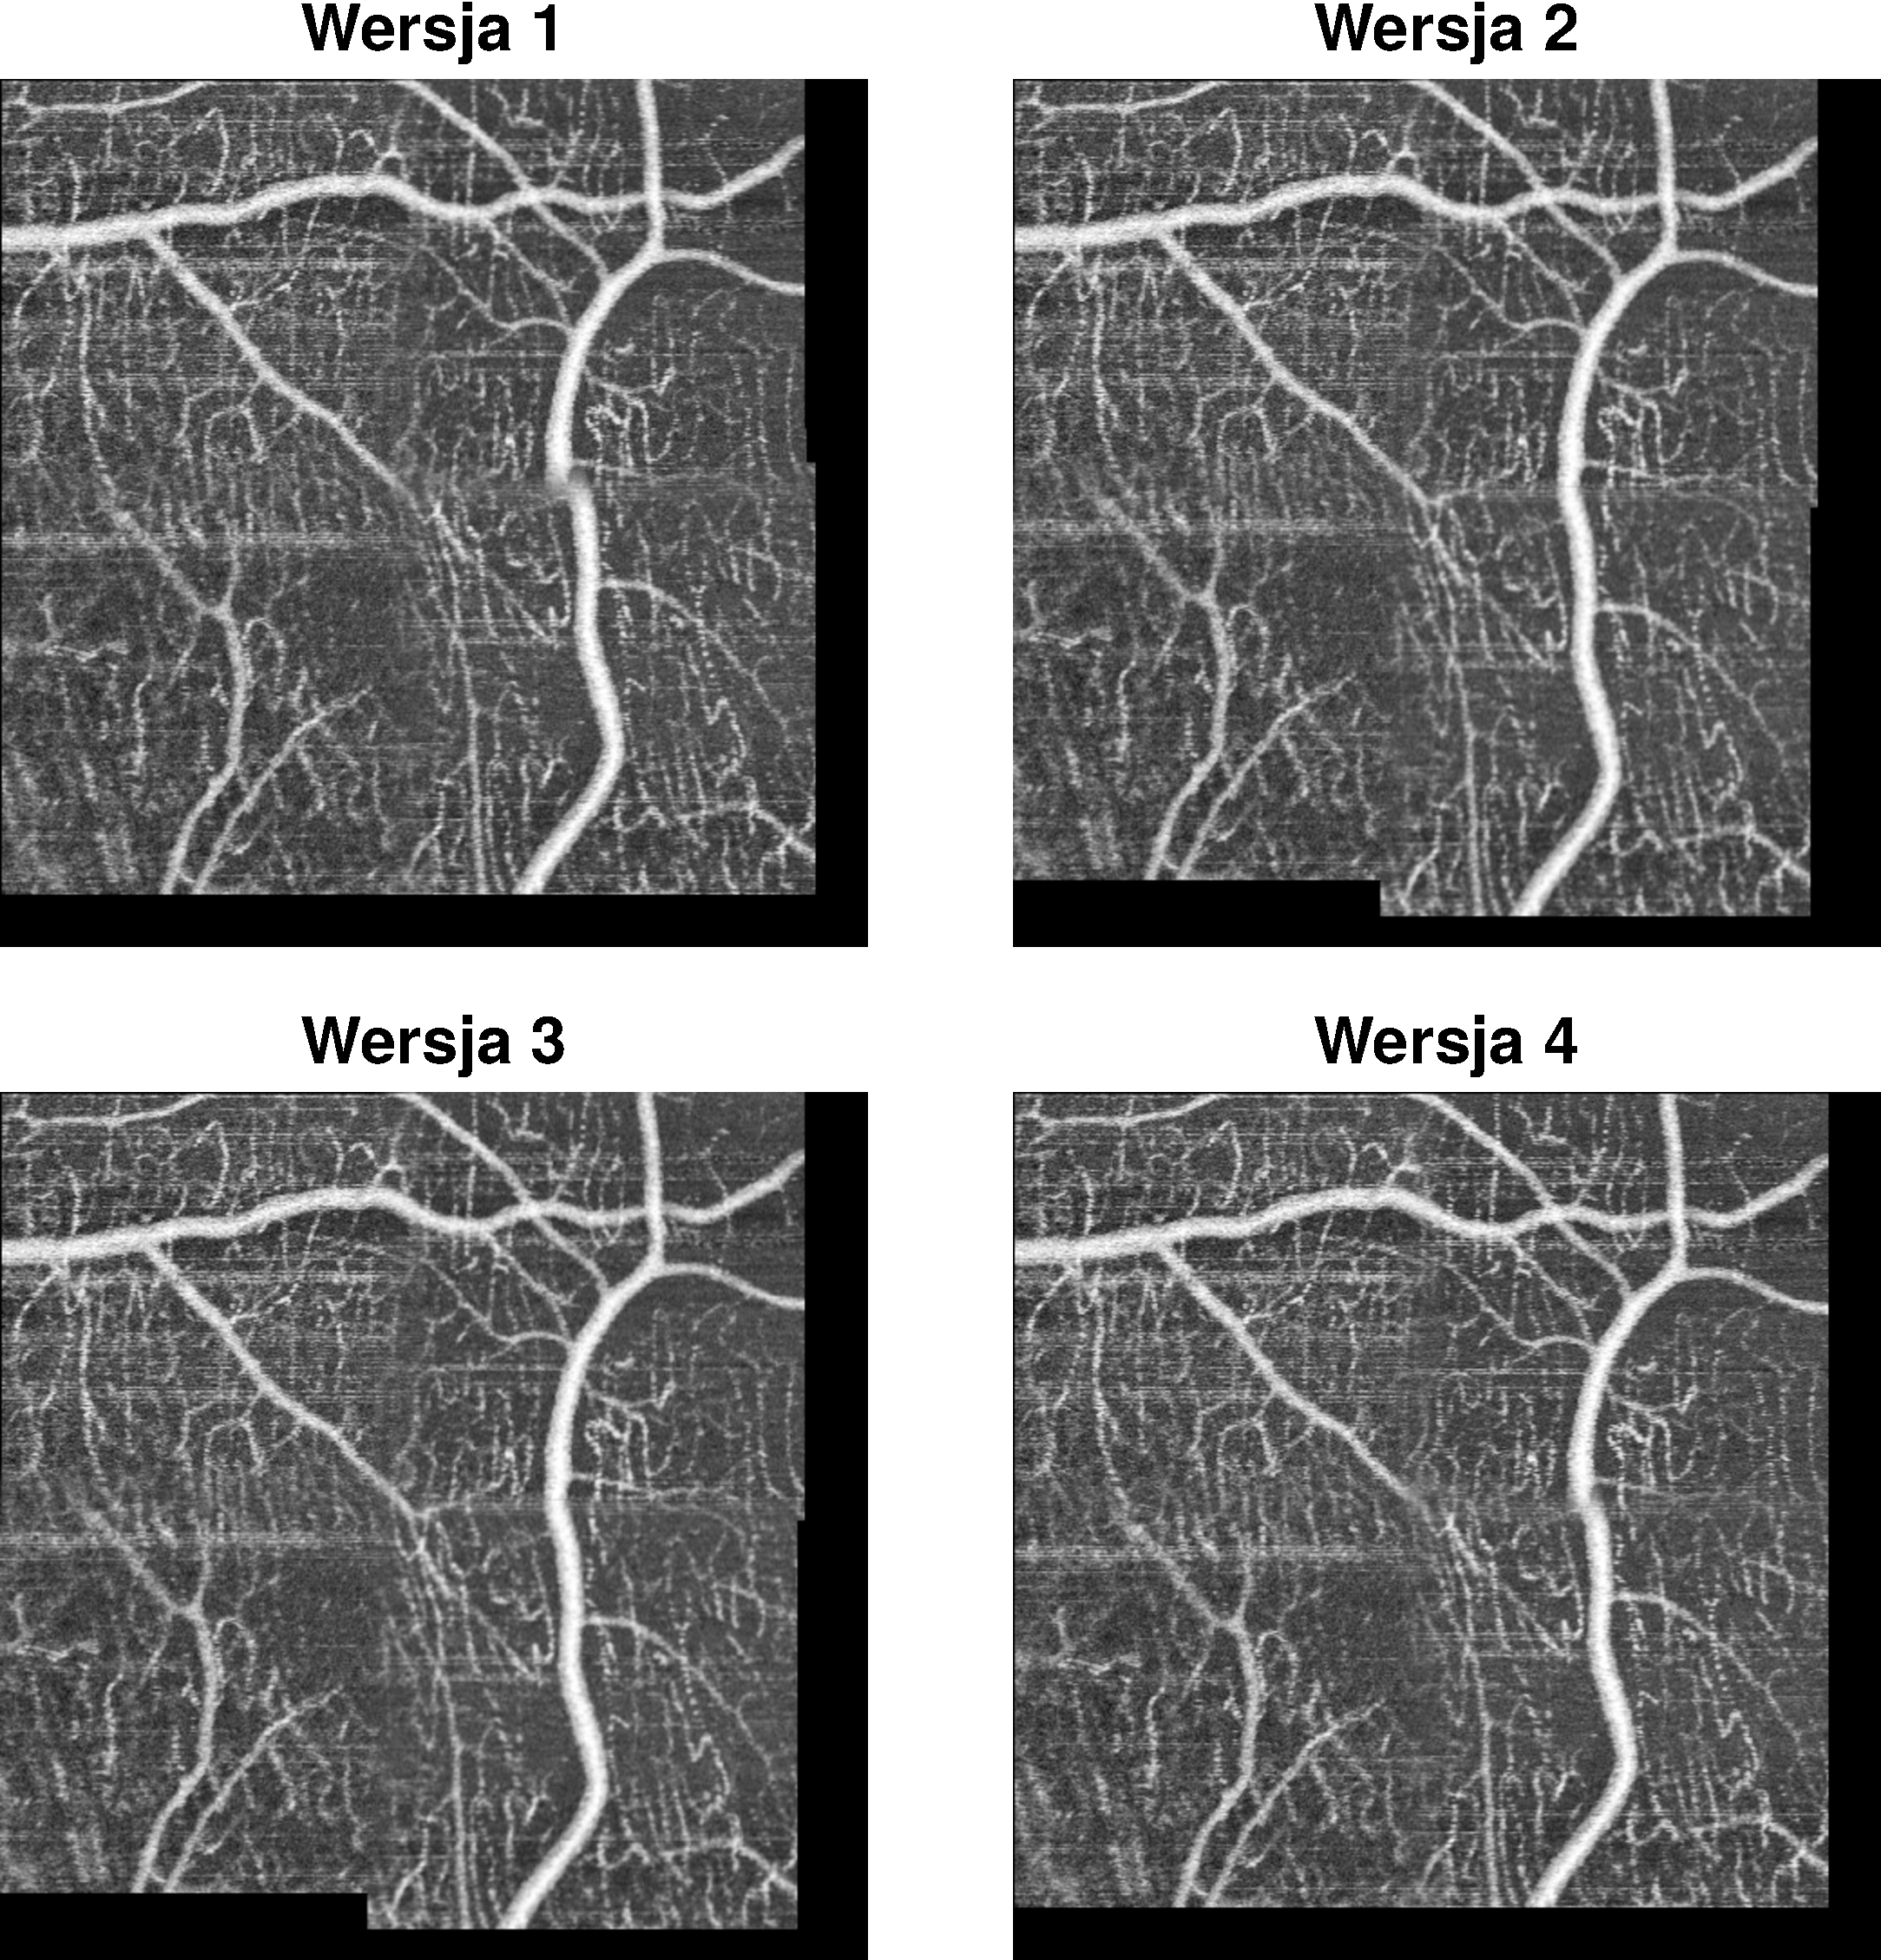
\includegraphics[width=10cm]{gfx/wynik_zbior_3}
  \caption{Cztery mozaiki będą wynikiem działania programu \texttt{mostitch} na zbiorze obrazów OCT z rysunku \ref{fig:wyniki_eksperymentow:zbior_3}.}
  \label{fig:wyniki_eksperymentow:wynik_zbior_3}
\end{figure}

\section{Ocena wyników}
\label{sec:ocena_wynikow}

Na podstawie zaprezentowanych wyników dla trzech przykładowych zbiorów trudno wybrać wersję sprawdzającą się dla każdego zbioru. Dla zbioru pierwszego z sekcji \ref{sec:zbior_1} najlepszą wersją jest wersja pierwsza, natomiast dla zbioru drugiego z sekcji \ref{sec:zbior_2} najlepiej prezentującym się wynikiem jest wersja druga. Dla zbioru trzeciego z sekcji \ref{sec:zbior_3} najlepiej wygląda mozaika z wersją drugą lub trzecią. 

Taka rozbieżność rezultatów dla różnych wartości parametrów jest głównym podowodem tworzenia czterech różnych wersji mozaik przez program \texttt{mostitch}. Dzięki takiemu rozwiązaniu osoba z wiedzą ekspercką jest w stanie stwierdzić, który obraz nadaje się najlepiej do wybranego zastosowania. Co więcej, otrzymanie czterech różnych wynikowych mozaik oszczędza czas uruchamiania programu z różnymi wartościami parametrów.













